\chapter{绪论}

\section{心电监护的意义}
21 世纪是生命科学的世纪,也是生物医学工程的世纪。生物医学信号的分析处理和生物医学仪器的研制开发是现代医学与保健养生中不可缺少的
重要组成部分。心血管疾病一直是危害人类健康、造成人类死亡的主要原因之一。在西方欧美发达国家,心血管疾病高发病率与高死亡率一直是危
害中老年人群健康的首要疾患。就我国自身而言,随着近些年人民生活水平的提高,心血管疾病的发病率和病死率同时呈逐年上升趋势。因此,一方面
我们应大力普及推广相应心血管疾病的预防及治疗基础原理与知识,另一方面亟需加强研究心脏处于不同病变状况下的生理电信号特性,
特别是通过人体导联实时无创的监测检测心脏的各项生理参数,并研制出对症治疗的医学仪器,辅助医生进行临床实际诊断。

自 1903 年心电图(electrocardiogram,ECG)引入医学临床以来,无论是在医学的临床治疗方面,还是在实际工程应用方面,心电信号诊断过程中的记录技术、
处理技术与诊断技术均得到长足的发展,并积累了相当丰富的资料。时至今日,在心脏疾病的临床诊断中心电图仍具有不可替代的参考价值,
它为医生对患者心脏疾病的正确分析、诊断、治疗和监护提供了客观指标。当前心电信号的处理仍然是生物医学工程界重要研究问题之一。
我国目前医疗水平不够发达,心电图自动分析和分类能够减轻心脏病专家的负担,并提高诊断速度,有着重要的临床意义与实际意义。

\section{心电监护的发展及现状}
对于心电的研究可以追溯到 18 世纪末、19 世纪初。最早由意大利解剖学家加尔瓦尼提出生物电的存在,1843 年德国生理学家雷蒙德证实了该理论的
正确性。13 年后 R.V.Koelliker首次在人体上检测到了心脏活动电位。1903 年,Einthoven 使用弦线电流计采集心电信号,开创了心电信号记录的新
纪元。从此,对心电图的研究进入了飞速发展的阶段。如今,心电图作为临床上常规的检查项目之一,诊断结果可靠,检测简单方便,而且对患者完全无
创伤,是临床上确诊心脏方面疾病的重要手段之一。

远程医疗是指通过计算机技术、通信技术与多媒体技术,同医疗技术相结合,旨在提高诊断与医疗水平、降低医疗开支、满足广大人民群众保健需求的
一项全新的医疗服务。而远程医疗在心电监测领域的应用要首推 20 世纪 50 年代美国人 Holter 发明的动态心电图机(Dynamic ECG,一般临床上简称为Holter)\cite{1}。
该动态心电监测仪器 Holter 可以实现长时间记录人在正常生活状态下的心电活动,对患者的异常心电进行检测。长期以来,Holter 一直是心血管疾病诊断领域重要的
检测手段,在临床诊断与其他医学研究方面得到了广泛应用。但是,Holter 仪器一般只能进行数据的采集工作,心电数据的分析工作必须在医院回收数据后进行,
在实时诊断方面有着先天的不足。

近些年来随着信息技术与网络技术的高速井喷式发展,特别是低成本的智能手机及全球性移动通信网络的普及,医疗信息化成为人们关注的焦点。在此背景下,
远程医疗的一个分支,移动医疗逐渐走入了人们的视线\cite{2}。移动医疗,即 Mobile Health,指的是使用移动通信技术,如 PDA 和智能手机等提供医疗服务和信息。目前移动医疗的
应用领域主要有紧急状况的处理、慢性疾病的长期监控以及为偏远地区就医提供帮助等。移动医疗的工作原理如\autoref{fig:101}所示。用户会佩戴一种轻量级的医疗监视系统——人体局域
网络(BAN),BAN 通过无线传感技术获取医疗数据,然后通过无线通信技术将信息传递给医院的医疗信息处理中心,供医生查看。

\begin{figure}[htbp]
    \centering
    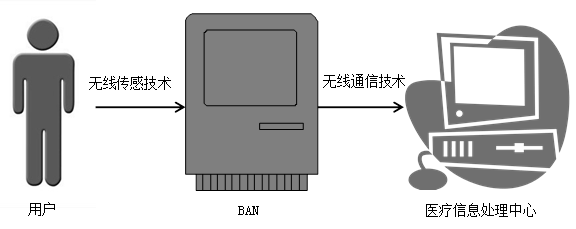
\includegraphics[width=.7\linewidth]{101}
    \caption{\label{fig:101}移动医疗服务相关技术}
\end{figure}

移动医疗跨界融合信息通讯和卫生医疗产业,具有很长的产业链\cite{3}。产业链上包括电信运营商、设备商、终端商、系统集成商、软件方案商等众多参与者。据美国市场研究公
司 RNCOS 的美国医疗保健信息技术市场报告分析,由 2011 年底算起,从 2012 年至 2014年,医疗保健信息技术产业开支将增长 24\% ,即 400 亿美元。该调查指出,目前美国每年
已有约 800 亿美元用于医疗保健信息技术产业,其中硬件构成该市场的 65\% ,紧跟其后的是软件和服务。在美国,移动医疗保健市场将在 2012~2014 年增长 22\% 左右。而在中国,
据业界人士预测,移动医疗目前带动的市场规模约在数十亿人民币。智能手机的普及为移动技术支持医疗服务提供关键基础。据国际电信联盟等组织统计,
目前约有 64\% 的智能手机用户都分布在发展中国家。预计到 2012 年,所有边远地区的居民将会有一半拥有移动通信设备。
德国市场研究公司 Research2guidance 预计到 2015年,在使用智能手机的用户中有三分之一以上的人将使用医疗保健类的移动应用程序。
移动医疗通过提供时间和空间的灵活性,使医疗保健系统更有效地配置资源,降低医疗服务成本,使更多人为之受益,具有广阔的发展前景。因此,本文设计基于移动医疗的
心电监护系统有着重要的行业前瞻意义。

\section{本文的主要工作及组织结构}
本文基于 Android 智能手机平台开发了一款心电检测分析系统应用软件,实现了对已经采集好的心电数据进行简单的滤波去噪、心电常用特征值提取、并对滤波前后数据的实
现了动态显示及简单的数据分析等功能。全文共分为五章,组织结构如下:

第一章是绪论,阐述了本文的研究背景、意义和国内外研究现状,并介绍了本文的组织结构。

第二章是 Android 集成环境的概述,按照 Android 的起源与发展、特点与优势、体系结构、组件及工作机制等顺序依次阐述了相应的背景,并在最后简单介绍了本文的开发环境。

第三章是心电信号的基础理论,主要介绍了心电的产生机理及特点,心电数据的基本特征及其生理意义,并对心电采集检测过程中易出现的干扰噪声做了相应的介绍。最后介
绍了本文分析的数据来源,即 MIT 的心电异常数据库。

第四章详细研究了心电监测系统中的关键方法和技术,包括去噪、特征提取等算法原理并对实际代码的进行了分析,此外,对去噪过程中的多种算法定性的给出了相应的
Matlab 仿真处理结果及滤波去噪效果的具体量化对比。

第五章是系统的设计和实现,首先探讨了系统需求、主要功能模块,其次简单介绍了软件模块 UI 界面的设计,再次对软件的动态显示处理前后的数据的工作原理做了相应的
介绍,最后详细介绍了系统的实现流程和最终代码实现,并给出了在智能手机上的运行效果。

最后是本文结论,总结了本文最后实际完成的主要工作与成果,分析了实际完成的系统的不足之处,并指出了下一步的研究方向。

\section{本章小结}
本章从心电监护的背景意义说起,介绍了心电监护的发展历史及现状,并对近些年来兴起的远程医疗与移动医疗做了简单的介绍。在最后概括了本文的工作,同时对本文的行
文结构做出了相应的介绍。